\chapter{Prace nad kodem źródłowym projektu (AK)}
\label{cha:code}

% setup
\graphicspath{{5_code/static/}}

Niniejszy rozdział stanowi opis wprowadzonych przez autorów zmian w kodzie źródłowym aplikacji \emph{ggss-runner}, stanowiącej trzon warstwy oprogramowania systemu GGSS. Opis poszczególnych modyfikacji poprzedzony został krótkim wprowadzeniem, opisującym wysokopoziomowe działanie omawianego programu oraz wynikające z jego specyfiki ograniczenia i założenia. Omówienie wprowadzonych zmian podzielone zostało na dwie części. W pierwszej z nich przedstawione zostały modyfikacje nie mające wpływu na sposób działania aplikacji, ale poprawiające jakość jej kodu źródłowego, np. poprzez jego migrację do nowszego standardu języka C++. Druga część stanowi natomiast opis nowych funkcjonalności oraz rozszerzeń wprowadzonych przez autorów do projektu. 

\section{Analiza aplikacji \emph{ggss-runner}}

\clearpage
\section{Specyfika i metodyka pracy}
Rozwój systemu działającego przez wiele lat w dedykowanym środowisku produkcyjnym, charakteryzującego się bardzo wysoką niezawodnością, wymagał od autorów dostosowania sposobu pracy w taki sposób, by wprowadzone zmiany nie miały negatywnego wpływu na jakość działania projektu. Wprowadzanie udoskonaleń w powstałym przed laty kodzie źródłowym niesie ze sobą dodatkowe wyzwania, wynikające m.in. ze sposobu, w jaki oryginalnie zaprojektowany został system (brak ogólnie przyjętych dziś praktyk programistycznych). Dlatego też pracując nad aplikacją \emph{ggss-runner}, autorzy zdecydowali się na przyjęcie szeregu ograniczeń i praktyk, mających na celu ułatwienie pracy z jej kodem źródłowym oraz utrzymanie jej wysokiej niezawodności, m.in. poprzez wczesne wykrywanie błędów. Należą do nich m.in.: wymóg przygotowywania testów jednostkowych (uruchamianych automatycznie w ramach procesu ciągłej integracji) dla każdego modyfikowanego lub tworzonego modułu projektu, dla którego było to możliwe, ograniczenie zakresu wprowadzanych zmian oraz wymóg, by każda wprowadzana zmiana, przed jej dołączeniem do gałęzi głównej danego modułu, poddawana była inspekcji wykonywanej przez pozostałych członków zespołu (tzw. \emph{code review}).


\subsection{Testy jednostkowe}
Celem testów jednostkowych jest sprawdzenie poprawności działania pojedynczego elementu systemu, rozumianego jako implementacja określonej funkcjonalności wchodzącej w skład logiki biznesowej projektu. Mówiąc inaczej, celem testów jednostkowych jest sprawdzenie zachowania testowanego komponentu (mogącego być, w zależności od konkretnego przypadku, pojedynczą funkcją, klasą czy też całym modułem), nie zaś weryfikacja szczegółów implementacyjnych. Powinny być one przygotowywane w ten sposób, by możliwe było ich automatyczne uruchomienie w celu weryfikacji każdej wprowadzanej przez programistę zmiany (np. po umieszczeniu nowej rewizji w portalu GitLab). 

Autorzy zdecydowali się na przygotowywanie testów jednostkowych dla każdego modyfikowanego komponentu wchodzącego w skład aplikacji \emph{ggss-runner}, dla którego istniała taka możliwość. Dzięki temu możliwe było sprawdzenie, w jaki sposób działał dany element projektu przed wprowadzeniem poprawek lub rozszerzeń, oraz czy dokonanie modyfikacji nie skutkowało nieoczekiwaną zmianą sposobu jego funkcjonowania. Projekt w swojej pierwotnej wersji nie posiadał żadnego zautomatyzowanego systemu testowania, a zatem konieczne było wprowadzenie go od podstaw (zarówno na poziomie systemu budowania, ciągłej integracji i dostarczania, jak i na poziomie kodu źródłowego). Motywacją do zastosowania tego typu podejścia był wymóg zachowania niezawodności aplikacji \emph{ggss-runner} oraz fakt, iż testy jednostkowe stanowią współcześnie szeroko stosowaną praktykę. 

W celu tworzenia testów jednostkowych autorzy wykorzystali bibliotekę \emph{Boost.Test}. Pozwala ona dokonywać sprawdzeń takich jak porównanie wartości zwracanej przez funkcję do wartości oczekiwanej czy weryfikacja rzucenia określonego typu wyjątku. Biblioteka ta oferuje zatem podstawowe funkcjonalności pozwalające na testowanie projektu, jednakże z punktu widzenia systemu GGSS jest ona wystarczająca. Jej dodatkową zaletą, istotną z punktu widzenia przyjętych podczas prac nad projektem ograniczeń, brak konieczności wprowadzania dodatkowych zewnętrznych zależności, ponieważ aplikacja \emph{ggss-runner} korzystała już w swojej pierwotnej wersji z pakietu Boost.

Na listingu \ref{lst:example_tests} przedstawione zostały dwa przykładowe testy jednostkowe przygotowane przez autorów podczas prac nad projektem. Testom poddawany jest wchodzący w skład biblioteki \emph{fifo-lib} szablon klasy \lstinline{QueueLimited}, którego zadaniem jest implementacja generycznej kolejki o określonym rozmiarze, po przekroczeniu którego usunięty zostaje najstarszy znajdujący się w niej element (funkcjonalność ta wykorzystywana jest w aplikacji \emph{ggss-runner} do przechowywania wyników kilku ostatnich pomiarów wykonanych za pomocą danego detektora słomkowego). Ponieważ celem przykładu jest zaprezentowanie mechanizmu testów jednostkowych, nie zaś sposobu działania testowanej kolejki, przedstawione na nim zostały bardzo proste sprawdzenia. Testy weryfikują, czy utworzona za pomocą domyślnego konstruktora struktura nie posiada żadnych elementów oraz czy próba pobrania elementu z pustej kolejki zakończy się rzuceniem wyjątku.

\lstinputlisting[
    language=C++, 
    caption={Przykład stworzonych na potrzeby projektu GGSS testów jednostkowych, weryfikujących poprawność działania podstawowych operacji wykonywanych na testowanym komponencie - w tym przypadku jest to szablon klasy implementującej kolejkę o ograniczonym rozmiarze.}, 
    label={lst:example_tests}
]{5_code/code_samples/example_tests.cpp}

W przypadku pierwszego z zaprezentowanych testów widoczne jest zastosowanie konstrukcji \lstinline{BOOST_CHECK_EQUAL}, sprawdzającej równość przekazanych do niej argumentów, co pozwala zweryfikować, że rozmiar utworzonej w domyślny sposób kolejki jest równy 0. W przypadku drugiego testu zastosowane zostało makro \lstinline{BOOST_CHECK_THROW} pozwalające zweryfikować, czy wykonanie przekazanego kodu powoduje wyrzucenie określonego typu wyjątku (tutaj: \lstinline{QueueLimited<int>::ReadEmptyQueueException}). Oczywiście zaprezentowany przykład nie wyczerpuje możliwości oferowanych przez zastosowaną bibliotekę, takich jak tworzenie wspólnych dla wielu testów konfiguracji (tzw. \emph{test fixtures}), pozwalających m.in. na zdefiniowanie pewnego stanu początkowego.

Jak wspomniano, zaletą testów jednostkowych jest możliwość wykonywania ich automatycznie, np. podczas wdrażania nowej rewizji w zdalnym repozytorium. Przykładem tego typu funkcjonalności jest technologia GitLab CI/CD, wspierająca proces ciągłej integracji i dostarczania. Mechanizm CI/CD zintegrowany został z projektem GGSS w ramach przygotowanej przez autorów pracy inżynierskiej (obejmował wtedy przede wszystkim proces automatycznego budowania poszczególnych komponentów systemu) oraz rozbudowany o możliwość wykonywania automatycznych testów w ramach niniejszej pracy magisterskiej. Rysunek \ref{fig:cicd_tests} przedstawia graficzną reprezentację procesu ciągłej integracji i dostarczania (tzw. \emph{pipeline}) zdefiniowanego dla wchodzącego w skład projektu repozytorium \emph{ggss-software-libs}. Zaprezentowany w tym przypadku proces składa się z dwóch etapów (ang. \emph{stages}), z czego drugi stanowi nowość wprowadzoną w ramach niniejszej pracy - wykonanie testów jednostkowych. 

\begin{figure}[H]
\centering
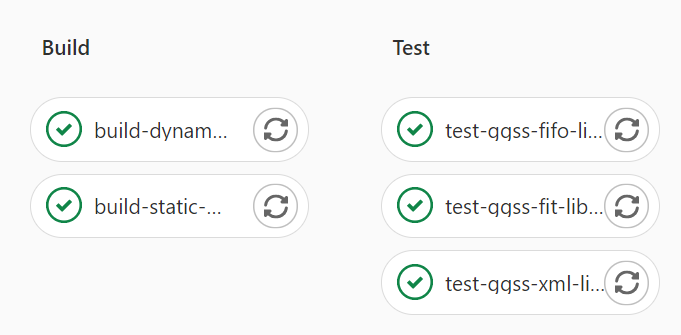
\includegraphics[width=0.6\textwidth]{pipeline.png}
\caption{Graficzna reprezentacja przebiegu procesu ciągłej integracji i dostarczania zdefiniowanego dla repozytorium \emph{ggss-software-libs}. Przeprowadzane działania podzielone zostały na dwa etapy, z czego drugi (\emph{Test}) odpowiada za automatyczne wykonanie znajdujących się w projekcie testów jednostkowych.}
\label{fig:cicd_tests}
\end{figure}

Z punktu widzenia testów jednostkowych interesujący jest problem weryfikacji działania komponentów posiadających zależności, których działanie może być różne w zależności od środowiska, w jakim uruchamiane są testy. Przykładem tego typu modułu może być biblioteka implementująca obsługę zasilaczy wysokiego napięcia z wykorzystaniem komponentu odpowiedzialnego za komunikację przy pomocy portu szeregowego. W zależności od tego, czy wspomniany zasilacz jest dostępny w środowisku testowym, zachowanie modułu odpowiedzialnego za komunikację będzie inne (zakończy się ona powodzeniem, lub też nie). W tym przypadku często stosowaną metodą jest wykorzystywanie tzw. atrap obiektów (ang. \emph{mock object}), mających na celu kontrolowane przez programistę symulowanie działania rzeczywistego obiektu. Z punktu widzenia aplikacji \emph{ggss-runner} zastosowanie tego podejścia było jednak w dużym stopniu problematyczne. Pierwszym powodem takiego stanu rzeczy jest fakt, iż wykorzystywana biblioteka \emph{Boost.Test} nie oferuje funkcjonalności wspierających tego typu metodyki testowania. Ponadto wymagają one tworzenia systemu w taki sposób, by możliwe było zastąpienie problematycznego obiektu jego atrapą - zwykle wykorzystuje się w tym celu wzorzec wstrzykiwania zależności (ang. \emph{dependency injection}) oparty o mechanizm polimorfizmu. System GGSS nie był jednak tworzony w sposób umożliwiający łatwe stosowanie tego wzorca, a jednocześnie przepisanie go w taki sposób wymagałoby bardzo znaczących nakładów pracy. Dlatego też zdecydowano się nie stosować w implementowanych testach podejścia opartego o atrapy. Nie miało to jednak znaczącego wpływu na możliwość implementacji testów automatycznych - problem pojawił się jedynie w przypadku jednego komponentu, odpowiedzialnego za obsługę wspomnianych zasilaczy. W tym konkretnym przypadku testy automatyczne zastąpione zostały bardzo szczegółowymi testami manualnymi w środowisku docelowym.

\subsection{Zakres wprowadzanych zmian} % napisac ze celem nie bylo przepisanie calej apki
Istotnym ograniczeniem przyjętym przez autorów podczas wykonywania prac nad projektem było ograniczenie zakresu możliwych do wprowadzenia zmian. Wprowadzanie zmian i nowych funkcjonalności do istniejącego systemu możliwe jest na wiele sposobów, w tym poprzez: 
\begin{itemize}
    \item pracę z istniejącą architekturą systemu, dostosowując do niej sposób implementacji wprowadzanych zmian
    \item przepisanie projektu (pełne lub dotyczące jedynie wybranych komponentów) na nową, nowocześniejszą architekturę
\end{itemize}
Ze względu na fakt, iż jednym ze stawianych przed systemem GGSS wymogów jest jego wysoka niezawodność, a ponadto charakteryzuje się on znaczącym poziomem skomplikowania (do jego pełnego zrozumienia wymagana jest wiedza domenowa z zakresu fizyki wykraczająca poza zakres niniejszej pracy) zdecydowano się postępować zgodnie z pierwszym z wymienionych podejść. Dlatego też wprowadzane przez autorów modyfikacje miały przede wszystkim charakter niewielkich, zwykle zamykających się w obrębie jednego lub dwóch modułów, zmian mających udoskonalić sposób działania systemu. 

\subsection{Przyjęte ograniczenia}
Poza do tej pory wspomnianymi, podczas prac nad rozwojem systemu GGSS autorzy stosowali szereg pomniejszych ograniczeń. Jednym z nich był brak możliwości wprowadzania do projektu jakichkolwiek nowych zależności zewnętrznych, aby nie komplikować sposobu jego budowania i dystrybucji. Ponadto istotnym było zachowanie zgodności projektu ze środowiskiem docelowym oraz zachowanie wstecznej kompatybilności z wcześniejszymi wersjami aplikacji \emph{ggss-runner}. Ostatni w wymienionych wymogów w sposób znaczący wpływał na sposób, w jaki implementowane był niektóre z nowych funkcjonalności - np. jeśli wprowadzony do aplikacji algorytm wymagał znajomości zdefiniowanej w pliku konfiguracyjnym wartości, nieobecnej tam w pierwotnej wersji projektu, to implementacja powinna przewidywać brak takiego parametru (np. poprzez zdefiniowanie wartości domyślnej). Ostatnim istotnym ograniczeniem był sposób, w jaki nowe zmiany integrowane mogły być z główną gałęzią danego modułu - wymagało to wykonania, przez innego niż osoba dokonująca zmian członka zespołu, inspekcji wprowadzonych modyfikacji.


\section{Poprawa jakości kodu źródłowego}
Niniejsza część pracy opisuje wybrane zmiany dokonane przez autorów w celu zwiększenia jakości kodu źródłowego wchodzącego w skład aplikacji \emph{ggss-runner} i wszystkich jej zależności. Opisane tu zmiany wykonywane były przede wszystkim w początkowym etapie prowadzonych prac, a ich celem, poza poprawą błędów czy unowocześnieniem kodu źródłowego, było umożliwienie autorom dokładnego zapoznania się ze strukturą projektu oraz zrozumienie zasady działania poszczególnych jego modułów oraz systemu jako całości. Proces wprowadzania do projektu opisanych modyfikacji wspomagany był przez wykorzystanie omówionych we wstępie teoretycznym narzędzi służących do przeprowadzania statycznej analizy kodu źródłowego. 

\subsection{Migracja do standardu C++11}
Jednym z celów niniejszej pracy była modernizacja kodu źródłowego aplikacji \emph{ggss-runner} poprzez przeprowadzenie jego migracji do standardu C++11, będącego najnowszym dostępnym w ramach wykorzystywanej infrastruktury wydaniem języka C++. Zastosowanie nowszego standardu miało na celu zwiększenie czytelności i bezpieczeństwa kodu źródłowego oraz wyeliminowanie, tam gdzie było to możliwe, zależności od bibliotek zewnętrznych, takich jak Boost. Przeprowadzone zmiany nie mogły stanowić jednak pełnej migracji - wynika to przede wszystkim z ograniczeń środowiska docelowego (stosowany tam kompilator nie wspiera standardu w pełni, np. nie jest możliwe poprawne wykorzystanie nagłówka \lstinline{<regex>}) oraz brak odpowiedników niektórych oferowanych przez Boost funkcjonalności, takich jak mechanizm slotów i sygnałów, w bibliotece standardowej.

Wprowadzane modyfikacje miały w większości charakter niewielkich, lokalnych zmian, niewywierających znaczącego wpływu na funkcjonalności implementowane przez poszczególne moduły projektu. Autorzy wprowadzili różnego typu usprawnienia w niemal każdym komponencie systemu, przez co niemożliwym jest zawarcie w pracy zestawienia prezentującego wszystkie poprawki. Dlatego też zdecydowano się na zaprezentowanie, w kolejnych akapitach niniejszej części manuskryptu, jedynie wybranego podzbioru wprowadzonych zmian, wzbogacając opis o przykłady w postaci fragmentów kodu pochodzących bezpośrednio z projektu. 

Jedną z najczęściej wprowadzanych modyfikacji było zastąpienie jawnie wykorzystującej mechanizm iteratorów pętli \lstinline{for} jej zakresowym odpowiednikiem. Zmiana ta, pomimo swojej prostoty, pozwala w sposób znaczący zredukować poziom skomplikowania niewielkiego fragmentu kodu. Pochodzący z biblioteki \emph{ggss-lib} przykład takiej zmiany zawarty został na listingach \ref{lst:for_before} (wersja oryginalna) oraz \ref{lst:for_after} (wersja po wprowadzeniu modyfikacji). Wynikowy fragment kodu jest krótszy, dzięki czemu pracującemu z nim programiście łatwiej skupić się na implementowanej logice biznesowej. Zastosowanie słowa kluczowego \lstinline{auto} pozwoliło ponadto uniknąć jawnego specyfikowania typu, na jakim wykonywane są operacje.

\lstinputlisting[
    language=C++, 
    caption={Fragment kodu źródłowego przed wprowadzeniem zmian: przykład zastosowania pętli \lstinline{for} wykorzystującej w sposób jawny pochodzący ze standardowej biblioteki szablonów mechanizm iteratorów.}, 
    label={lst:for_before}
]{5_code/code_samples/for_loop_before.cpp}

\lstinputlisting[
    language=C++, 
    caption={Fragment kodu źródłowego po wprowadzeniu zmian: przykład zastosowania zakresowej pętli \lstinline{for} oraz słowa kluczowego \lstinline{auto} w celu zwiększenia czytelności oraz skrócenia fragmentu kodu zaprezentowanego na listingu \ref{lst:for_before}.}, 
    label={lst:for_after}
]{5_code/code_samples/for_loop_after.cpp}

Ponadto zastąpiono znane z języka C typy wyliczeniowe (\lstinline{enum}) ich nowocześniejszym odpowiednikiem - silnymi typami wyliczeniowymi (\lstinline{enum class/struct}). Na listingu \ref{lst:enum_before} zamieszczony został pochodzący z biblioteki \emph{log-lib} fragment kodu, przedstawiający wykorzystanie starszej konstrukcji. Jej zastosowanie wiąże się z szeregiem wad, m.in. nie definiuje ona nowego zakresu, przez co zawarte w niej nazwy mogą potencjalnie tworzyć konflikt np. z innym typem wyliczeniowym. Znane z języka C rozwiązanie pozwala zatem na stosowanie zapisu \lstinline{int x = trace} - tzn. nie jest konieczne wyspecyfikowanie nazwy typu wyliczeniowego. Przedstawiony przykład obrazuje jeszcze jedną niedogodność związaną z wykorzystywaniem typów wyliczeniowych - możliwość przeprowadzania niejawnych konwersji do typu całkowitoliczbowego, by np. wykorzystać go w formie indeksu tablicy. Pomimo, że daje do programiście dodatkowe możliwości, do komplikuje tworzony kod poprzez dodanie do niego niewidocznych na pierwszy rzut oka przekształceń, co w wielu przypadkach uważane jest za złą praktykę, ponieważ jest sprzeczne z ideą tzw. \emph{samodokumentującego się kodu}.

\lstinputlisting[
    language=C++, 
    caption={Fragment kodu źródłowego przed wprowadzeniem zmian: przykładowe wykorzystanie typu wyliczeniowego - widoczna możliwość dokonania niejawnej konwersji do typu całkowitoliczbowego.}, 
    label={lst:enum_before}
]{5_code/code_samples/enum_before.cpp}

Listing \ref{lst:enum_after} przedstawia analogiczny fragment kodu, wykorzystujący silne typy wyliczeniowe. W stosunku do poprzedniego przykładu, w tym przypadku jawnie przypisano oczekiwane wartości do każdego z wystąpień w wyliczeniu - dzięki temu stosowanie ich jako indeksów tablicy jest bezpieczniejsze. Ponadto konieczna jest jawna konwersja do typu całkowitoliczbowego, wykonana za pomocą operatora \lstinline{static_cast}. Stosując silne typy wyliczeniowe programista nie stwarza możliwości wystąpienia konfliktu nazw, ponieważ definiują one nowy zakres. Zatem, by uzyskać wartość liczbową, należy wykonać operację \lstinline{int x = static_cast<int>(SeverityLevel::trace)}.

\lstinputlisting[
    language=C++, 
    caption={Fragment kodu źródłowego po wprowadzeniu zmian: wykorzystanie silnego typu wyliczeniowego, uniemożliwiającego niejawną konwersję do typu całkowitoliczbowego.}, 
    label={lst:enum_after}
]{5_code/code_samples/enum_after.cpp}

Autorzy zdecydowali się ponadto na wyeliminowanie z kodu źródłowego przestarzałych konstrukcji i zastąpienie ich odpowiednikami dostarczanymi przez standard C++11. Przykładem tego typu 
modyfikacji było zastąpienie, w kontekście tzw. dynamicznej specyfikacji wyjątków, słowa kluczowego \lstinline{throw} za pomocą specyfikatora \lstinline{noexcept}. Celem stosowania tych konstrukcji jest wskazanie intencji programisty na temat tego, czy stworzona funkcja może (pośrednio lub bezpośrednio) rzucić wyjątek. Pozorną zaletą specyfikatora \lstinline{throw} była ponadto możliwość zawarcia w kodzie informacji na temat typów rzucanych przez funkcję wyjątków. W rzeczywistości jednak stosowanie go ograniczało możliwości rozszerzania i modyfikacji kodu, ponieważ mogło spowodować krytyczny błąd w działaniu programu - jeśli rzucony został wyjątek inny, niż zostało zadeklarowane, to wykonanie programu było przerywane. Z tego też powodu jedynym stosunkowo bezpiecznym sposobem na wykorzystanie tej konstrukcji było wyspecyfikowanie, czy dana funkcja rzuca jakiekolwiek wyjątki. Ta sama funkcjonalność możliwa jest do uzyskania z wykorzystaniem wprowadzonego w standardzie C++11 specyfikatora \lstinline{noexcept} - pozwala on zawrzeć w deklaracji funkcji binarną informację na temat możliwości wyrzucenia wyjątku, a ponadto wspiera możliwość jej ewaluacji w czasie kompilacji. Przykład zastosowania zawarty został na pochodzącym z biblioteki \emph{caenn1470-lib} listingu \ref{lst:noexcept}. 

\lstinputlisting[
    language=C++, 
    caption={Przykład zastosowania specyfikatora \lstinline{noexcept} w kodzie projektu GGSS w celu zadeklarowania, że zaprezentowana metoda nie powinna rzucać wyjątków.}, 
    label={lst:noexcept}
]{5_code/code_samples/noexcept.cpp}


Standard C++11 wprowadza ponadto możliwość stosowania tzw. domyślnej inicjalizacji składowych (ang. \emph{default member initialization}), co pozwala nadawać domyślne wartości niestatycznym polom klasy, dzięki czemu możliwe jest uproszczenie istniejących w projekcie klas, np. poprzez likwidację niektórych konstruktorów. Na listingu \ref{lst:init_before} przedstawiona została uproszczona (pominięte zostały niektóre pola) struktura \lstinline{CaenHVParams}, pochodząca z biblioteki \emph{caenhv-lib} w wersji zgodnej ze standardem C++03. Widoczny jest zdefiniowany w klasie konstruktor, którego celem jest nadanie wartości składowym tworzonego obiektu, zarówno za pomocą listy inicjalizacyjnej, jak i znajdującej się w jego ciele pętli \lstinline{for}.


\lstinputlisting[
    language=C++, 
    caption={Fragment kodu źródłowego przed wprowadzeniem zmian: inicjalizacja niestatycznych składowych struktury za pomocą konstruktora.}, 
    label={lst:init_before}
]{5_code/code_samples/init_before.cpp}


Na listingu \ref{lst:init_after} zaprezentowany został natomiast analogiczny kod napisany z wykorzystaniem standardu C++11. Wynikowa struktura jest znacznie prostsza od swojej pierwotnej wersji, przede wszystkim za sprawą zastąpienia inicjalizacji składowych na poziomie konstruktora przez inicjalizację domyślną. Ponadto w swojej finalnej postaci struktura znacznie lepiej dokumentuje swoje przeznaczenie - jest to prosty, nieposiadający żadnych metod implementujących logikę, agregat. 

\lstinputlisting[
    language=C++, 
    caption={Fragment kodu źródłowego po wprowadzeniu zmian: zastosowanie domyślnej inicjalizacji niestatycznych składowych struktury.}, 
    label={lst:init_after}
]{5_code/code_samples/init_after.cpp}

Zaprezentowane do tej pory zmiany stanowią oczywiście jedynie wybrany podzbiór wykonanych przez autorów modyfikacji. Poza do tej pory opisanymi, wykonane zostały inne przekształcenia mające na celu migrację kodu źródłowego do standardu C++11, m.in.:
\begin{itemize}
    \item zastosowanie słowa kluczowego \lstinline{override} w celu jawnego zadeklarowania, że metoda znajdująca się w klasie pochodnej przeciąża metodę z klasy bazowej - pozwala to wykrywać na etapie kompilacji błędy związane z nieprawidłową implementacją polimorfizmu, takie jak zmiana sygnatury metody w klasie bazowej przy jednoczesnym niewykonaniu tej czynności w klasie pochodnej
    \item zastosowanie słowa kluczowego \lstinline{final} w celu zabronienia dziedziczenia lub przeciążania metod w przypadku modułów, które nie były projektowane z myślą o polimorfizmie
    \item zastąpienie opartej o pakiet Boost (m.in. \lstinline{boost::assign}) inicjalizacji kontenerów wchodzących w skład biblioteki standardowej za pomocą rozwiązań oferowanych przez standard C++11 (jednolita inicjalizacja i konstruktory oparte o \lstinline{std::initializer_list})
    \item zastąpienie, tam gdzie było to możliwe, znanych z języka C tablic za pomocą kontenera \lstinline{std::array}
    \item zastąpienie przygotowanych na potrzeby systemu GGSS funkcji, takich jak wykonująca konwersję typu liczbowego do łańcucha znaków funkcja pomocnicza \lstinline{toString}, za pomocą rozwiązań standardowych (np. \lstinline{std::to_string})
    \item zastosowanie semantyki przenoszenia i referencji do r-wartości
    \item zastąpienie słowa kluczowego \lstinline{typedef} za pomocą słowa \lstinline{using}
\end{itemize}

\clearpage
\subsection{Naprawa błędów w kodzie źródłowym}
Kod źródłowych wchodzący w skład warstwy oprogramowania systemu GGSS od początku prac charakteryzował się bardzo wysoką poprawnością - zawierał tak naprawdę jedynie niewielką liczbę niezagrażających działaniu systemu niedociągnięć. Celem autorów była poprawa działania tych fragmentów kodu, w których udało się zlokalizować wszelkiego typu niedoskonałości. 

Przeważająca część znajdowanych przez autorów, zarówno podczas oględzin kodu, jak i testów systemu w środowisku docelowym, błędów dotyczyła nietypowych scenariuszy, nie mających miejsca w czasie regularnego działania projektu. Bardzo często odnajdywane niedoskonałości związane były ze stosowanym w projekcie mechanizmem wielowątkowości - ich naprawa sprowadzała się zwykle do przeprowadzenia szczegółowych testów mających na celu identyfikację przyczyny i dokładnego miejsca występowania problemu oraz wprowadzenia niewielkiej poprawki (np. poprzez wykorzystanie dodatkowej zmiennej pomocniczej lub instrukcji warunkowej) w odpowiednim miejscu kodu źródłowego. Jednym z przykładów tego typu błędów była sytuacja, w której użytkownik próbował zmienić kolejność, w jakiej dokonywany jest pomiar za pomocą poszczególnych detektorów słomkowych, w trakcie trwania takiego pomiaru. W odpowiednich warunkach mogło to doprowadzić do sytuacji, w której zebrane dane przypisywane były do nieprawidłowego detektora. Dla przykładu, jeśli system skonfigurowany był w taki sposób, że pomiary dokonywane były kolejno dla detektorów o numerach \lstinline{1, 3, 6, 2}, a użytkownik, podczas pomiaru na detektorze \lstinline{3} dokonał zmiany kolejności na \lstinline{1, 4, 5, 2}, to wynik pomiaru wykonanego za pomocą detektora \lstinline{3} przypisywany był detektorowi o numerze \lstinline{4}. Ponieważ rozwiązywanie tego typu problemów wymagało przede wszystkim znajomości trudnych do przedstawienia w pracy magisterskiej detali dotyczących implementacji poszczególnych funkcjonalności systemu GGSS, autorzy zdecydowali się nie prezentować w niniejszym manuskrypcie szczegółów postępowania w tego typu przypadkach.

Zadaniem autorów było ponadto diagnozowanie i naprawianie usterek związanych niepoprawną implementacją algorytmów wchodzących w skład projektu. Podczas prac nad kodem źródłowym aplikacji \emph{ggss-runner} zidentyfikowany został jeden tego typu problem, związany z działaniem odpowiedzialnej za przetwarzanie plików konfiguracyjnych systemu GGSS biblioteki \emph{xml-lib}.


% wspomniec, ze bledow bylo bardzo niewiele, zaden z nich nie zagrazal tak naprawde poprawnosci dzialania projektu
% jako przyklad opisac blad z wyszukiwaniem w XML-u

\subsection{Likwidacja nieużywanych fragmentów kodu źródłowego}
% fragmenty takie jak w fit-lib (3 znalezione funkcje) i xml-lib (dwie implementacje przechowywania wezlow) - pozostałosci po starszych wersjach systemu i eksperymentach
% pozostalosci po starej wersji systemu w bibliotece ggss-lib
% szczegolny przyklad: metody lamiace enkapsulacje w bibliotece fifo-lib

\subsection{Pozostałe zmiany i podsumowanie}
% zmiana w strukturze bibliotek (rozbicie na pliki - log i sigslot)
% wyodrebnienie powtarzajacych sie fragmentow kodu (np. w log-lib i xml-lib)
% wspomniec ze ujednolicona zostala konwencja nazewnictwa i dokumentacji
% eliminacja wykomentowanego kodu, poprawienie formatowania (przyklad z xml jako jpg)
% podsumowanie - ile bibliotek poddanych zostalo refactoringowi, ktore nie i dlaczego

\clearpage
\section{Rozszerzenie możliwości aplikacji}
Zadaniem autorów, poza poprawą działania i jakości systemu GGSS, było wzbogacenie go o nowe funkcjonalności. W tej części pracy przedstawiony został szczegółowy opis najważniejszych rozszerzeń wprowadzonych przez autorów do aplikacji \emph{ggss-runner}. 

\subsection{Obsługa zaawansowanych komend dla zasilaczy wysokiego napięcia} \label{ch:hv}
Jednym z zadań systemu GGSS jest komunikacja z zasilaczami wysokiego napięcia w celu monitorowania oraz modyfikacji ich parametrów. W swojej aktualnej postaci projekt wykorzystuje trzy czterokanałowe zasilacze CAEN N1470, których zadaniem jest dostarczanie zasilana do słomkowych liczników proporcjonalnych. Urządzenia podłączone są do głównego komputera łańcuchowo (ang. \emph{daisy chain}), tzn. pierwszy zasilacz podłączony jest do niego bezpośrednio, a każdy kolejny łączony jest z poprzednim (rys. \ref{fig:psu0}). Komunikacja z urządzeniami odbywa się poprzez port szeregowy, za pomocą specjalnych komend, których składnia określona została przez producenta. 

\begin{figure}[H]
\centering
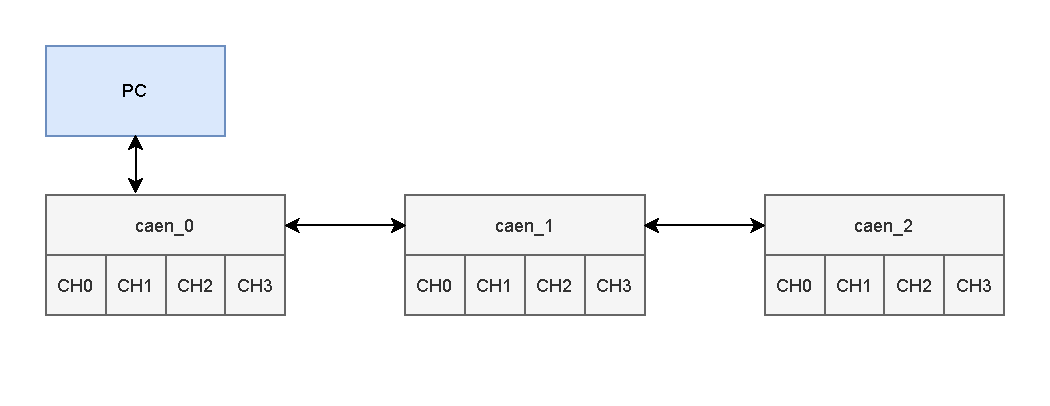
\includegraphics[width=\textwidth]{hv_psu_0.pdf}
\caption{Łańcuchowe połączenie trzech czterokanałowych zasilaczy wysokiego napięcia z komputerem. Za pomocą kwadratów z oznaczeniem \lstinline{CH<N>} przedstawiono kanały każdego z urządzeń. Nazwy poszczególnych modułów zostały, na potrzeby przykładu, uproszczone względem tych stosowanych w systemie GGSS.}
\label{fig:psu0}
\end{figure}

Dostarczone przez producenta zasilaczy komendy sterujące pozwalają zarówno na monitorowanie (MON), jak i modyfikację (SET) parametrów urządzeń, takich jak oczekiwana wartość napięcia. Poza wykonywaną operacją, komendy różnią się od siebie ponadto zakresem działania - mogą dotyczyć poszczególnych kanałów (np. modyfikacja maksymalnej dopuszczalnej wartości napięcia) lub modułu jako całości (np. pobranie jego numeru seryjnego). Przykładowo, format komendy monitorującej wartość określonego parametru dla pojedynczego kanału zdefiniowany został przez producenta w następujący sposób: \lstinline{$BD:<moduł>,CMD:MON,CH:<kanał>,PAR:<parametr>}. Dostępne polecenia pozwalają wykonywać operacje tylko ja jednym module jednocześnie, możliwy jest natomiast wybór pomiędzy jednym kanałem, a wszystkimi (specjalna wartość 4). System GGSS w swojej pierwotnej wersji oferował obsługę tego typu komend, stanowiąc pośrednika między użytkownikiem a urządzeniami.

Stosowanie tego typu poleceń charakteryzuje się, z punktu widzenia użytkownika, pewnymi niedogodnościami, z czego najważniejsze to: brak możliwości operowania na kilku zasilaczach jednocześnie oraz trudna do zapamiętania, nieintuicyjna składnia. Zadaniem autorów było przygotowanie biblioteki udostępniającej alternatywny, przyjazny użytkownikowi, zestaw komend, który byłby następnie tłumaczony przez system GGSS na format zdefiniowany przez producenta urządzeń. 

W przypadku komend monitorujących parametry na poziomie poszczególnych kanałów przygotowany został następujący format: \lstinline{hv <moduł>:<kanał> mon <parametr[,inne_parametry]>}, przy czym możliwe jest zastosowanie znaku \lstinline{*} w zamian za specyfikację modułu lub kanału, co oznacza \emph{wszystkie moduły/kanały}. Ponadto, dodatkowym ulepszeniem w stosunku do oryginalnej składni jest możliwość monitorowania wartości kilku parametrów jednocześnie - w takim wypadku należy przedzielić je przecinkiem. Przykładem nowego polecenia jest \lstinline{hv *:2 mon vmon}, które pozwala na monitorowanie napięcia (parametr \lstinline{vmon}) na kanale numer 2 dla każdego z zasilaczy (rys. \ref{fig:psu1}). To polecenie jest odpowiednikiem wykonania trzech, zgodnych z oryginalna składnią, komend (po jednej dla każdego modułu):
\begin{lstlisting}
$BD:0,CMD:MON,CH:2,PAR:VMON
$BD:1,CMD:MON,CH:2,PAR:VMON
$BD:2,CMD:MON,CH:2,PAR:VMON
\end{lstlisting}

\begin{figure}[H]
\centering
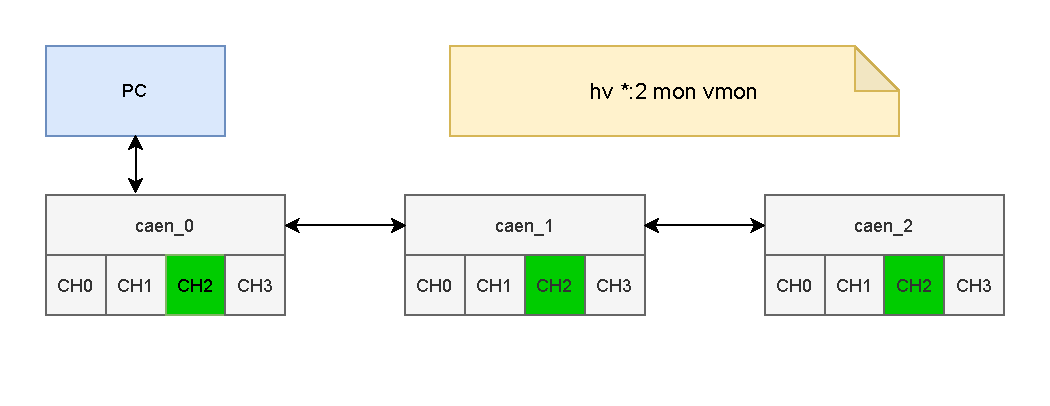
\includegraphics[width=\textwidth]{hv_psu_1.pdf}
\caption{Zasada działania komendy typu \lstinline{hv *:2 mon <parametry>} - kolorem zielonym oznaczone zostały te kanały zasilaczy, z których pobrana zostanie monitorowana wartość. W tym przypadku jest to kanał numer 2 w każdym z urządzeń.}
\label{fig:psu1}
\end{figure}

Odpowiedź otrzymana od urządzeń formatowana jest w taki sposób, by możliwe było stosunkowo łatwe jej parsowanie (np. w celu tworzenia skryptów). Przykładowy wynik działania dla zaprezentowanej wyżej komendy prezentuje się następująco:
\begin{lstlisting}
OK: caen_0:2:VMON:1364.8;caen_1:2:VMON:0.0;caen_2:2:VMON:0.0
\end{lstlisting}

Innym przykładem wspieranej komendy jest \lstinline{hv caen_1:* mon vmon} - dokonuje ona sprawdzenia wartości napięcia na wszystkich kanałach zasilacza oznaczonego nazwą \lstinline{caen_1}. Jej odpowiednikiem zapisanym za pomocą składni dostarczonej przez producenta byłoby polecenie \lstinline{$BD:1,CMD:MON,CH:4,PAR:VMON} - wartość 4 pełni tutaj rolę wartości specjalnej, odnoszącej się do wszystkich kanałów. Autorzy zdecydowali się jednak nie stosować tej konwencji (zastępując wartość 4 znakiem \lstinline{*}), ponieważ dla osoby nieznającej szczegółów działania zasilaczy CAEN N1470 mogłaby być ona myląca, a ponadto tworzyłaby ona powiązanie pomiędzy ilością kanałów w zasilaczu, a logiką biblioteki implementującej obsługę komend. Zasada działania powyższej komendy zaprezentowana została w formie graficznej na rysunku \ref{fig:psu2}.

\begin{figure}[H]
\centering
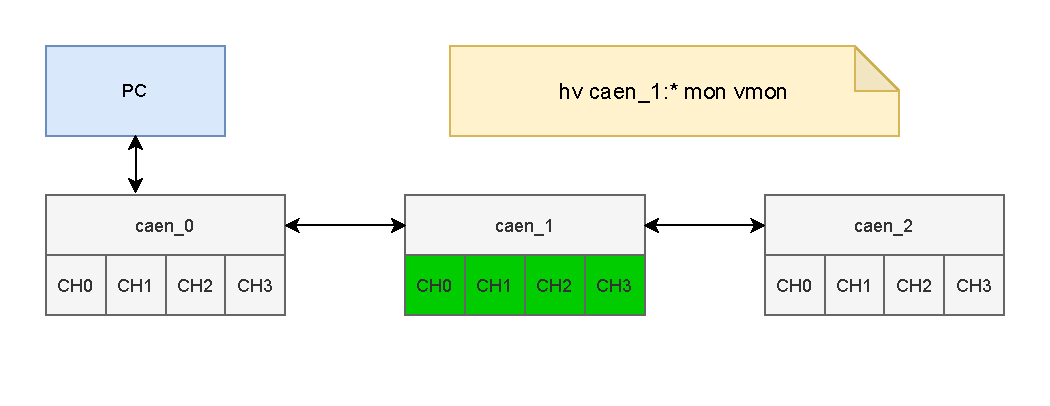
\includegraphics[width=\textwidth]{hv_psu_2.pdf}
\caption{Zasada działania komendy typu \lstinline{hv caen_1:* mon <parametry>} - kolorem zielonym oznaczone zostały te kanały zasilaczy, z których pobrana zostanie monitorowana wartość. W tym przypadku są to wszystkie kanały urządzenia o nazwie \lstinline{caen_1}.}
\label{fig:psu2}
\end{figure}

Zadaniem przygotowanych komend jest ułatwienie użytkownikowi prowadzenia interakcji z zasilaczami wysokiego napięcia za pośrednictwem systemu GGSS. Ich stosowanie pozwala, za pomocą jednego polecenia, wykonać zapytanie wymagające wcześniej zastosowania większej liczby komend. Np. komenda \lstinline{hv *:* mon vset,vmon,iset}, dokonująca sprawdzenia wartości trzech różnych parametrów dla każdego kanału we wszystkich urządzaniach, odpowiada wykonaniu dziewięciu poleceń za pomocą składni dostarczonej przez producenta:
\begin{lstlisting}
$BD:0,CMD:MON,CH:4,PAR:VMON
$BD:1,CMD:MON,CH:4,PAR:VMON
$BD:2,CMD:MON,CH:4,PAR:VMON
$BD:0,CMD:MON,CH:4,PAR:VSET
$BD:1,CMD:MON,CH:4,PAR:VSET
$BD:2,CMD:MON,CH:4,PAR:VSET
$BD:0,CMD:MON,CH:4,PAR:ISET
$BD:1,CMD:MON,CH:4,PAR:ISET
$BD:2,CMD:MON,CH:4,PAR:ISET
\end{lstlisting}

W podobny sposób przygotowana została składnia komend wykonujących operacje na poziomie pojedynczego modułu - użytkownik pomija jedynie informację o wybranych kanałach. Tego typu komendy pozwalają uzyskiwać informacje takie jak nazwa modułu czy też jego numer seryjny. Przykładem polecenia operującego na poziomie zasilaczy jest \lstinline{hv * mon bdname} pobierające nazwy wszystkich trzech modułów - jego zasada działania zilustrowana została na rysunku \ref{fig:psu3}. Jest to odpowiednik wykonania trzech komend za pomocą składni dostarczonej przez producenta (po jednej dla każdego urządzenia).

\begin{figure}[H]
\centering
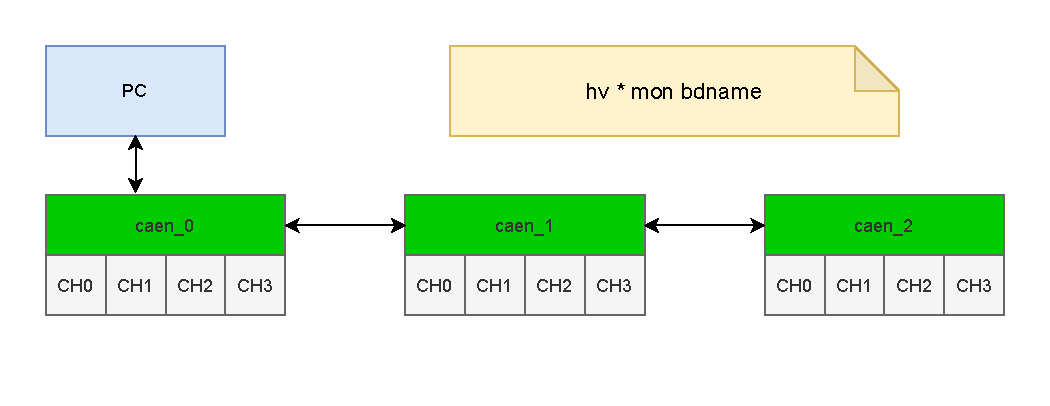
\includegraphics[width=\textwidth]{hv_psu_3.pdf}
\caption{Zasada działania komendy typu \lstinline{hv * mon <parametry>}, tzn. operującej na poziomie modułów. Kolorem zielonym oznaczone zostały te zasilacze, z których pobrana zostanie monitorowana wartość - w tym przypadku, ze względu na wykorzystanie znaku \lstinline{*}, są to wszystkie dostępne moduły.}
\label{fig:psu3}
\end{figure}

Autorzy przygotowali ponadto komendy typu SET, pozwalające na modyfikowanie wartości parametrów, zarówno na poziomie pojedynczych kanałów, jak i zasilaczy. Ich zasada działania jest bardzo podobna do komend monitorujących, z kilkoma różnicami:
\begin{itemize}
    \item użytkownik po nazwie parametru specyfikuje jego oczekiwaną wartość
    \item nie ma możliwość wykonywania komendy dla kilku parametrów jednocześnie
\end{itemize}
Przykładem tego typu polecenia, wykonującego operację zmiany wartości napięcia na każdym kanale zasilacza \lstinline{caen_0} na wartość 0, jest komenda \lstinline{hv caen_0:* set vset 0}. Sposób określania wykorzystywanych zasilaczy i kanałów jest identyczny do tego stosowanego w przypadku komend typu MON. Szczególnym przypadkiem komend typu SET są komendy typu \lstinline{hv <moduł>:<kanał> set ON/OFF}, których zadaniem jest włączenie lub wyłączenie danego kanału - w ich przypadku użytkownik nie specyfikuje wartości.

W celu zachowania możliwości wykorzystywania składni przygotowanej przez producenta zasilaczy, wprowadzony został trzeci typ polecenia, oznaczany za pomocą słowa RAW. Składnia tego typu poleceń jest następująca: \lstinline{hv <moduł> raw <polecenie>}, gdzie \lstinline{<polecenie>} oznacza komendę zgodną z oryginalną składnią. Przykładem komendy typu RAW jest polecenie \lstinline{hv caen_0 raw $BD:00,CMD:MON,CH:0,PAR:VMON}, monitorujące wartość napięcia na kanale numer 0 urządzania o nazwie \lstinline{caen_0}. Komendy te pozwalają operować jednocześnie jedynie na jednym urządzeniu - wynika to z faktu, iż specyfikacja \lstinline{<moduł>} musi być zgodna z numerem zawartym w ciele komendy.

Z punktu widzenia implementacji zaprezentowana funkcjonalność przygotowana została w formie, znajdującej się w repozytorium \emph{ggss-hardware-libs}, biblioteki statycznej \emph{hvcommand-lib}. Zawarty w niej kod przygotowany został zgodnie ze standardem C++11 i oparty został o polimorficzną hierarchię klas reprezentujących parsery, z których każdy przystosowany został do przetwarzania innego typu komend: MON, SET lub RAW (rys. \ref{fig:psu_parsers}). Odpowiednia implementacja wybierana jest na podstawie trzeciego elementu każdej z komend (podział na elementy za pomocą białych znaków) - służy do tego klasa \lstinline{HighVoltageCommandParserFactory}. Następnie parser przekształca otrzymaną komendę do zbioru obiektów reprezentujących czynności wykonywane na urządzeniach - kontener ten określony jest w kodzie źródłowym nazwą \lstinline{HighVoltageCommandQueue}. W kolejnym kroku poszczególne akcje są wykonywane, a wynik jest przekształcany do odpowiedniego formatu.

\begin{figure}[H]
\centering
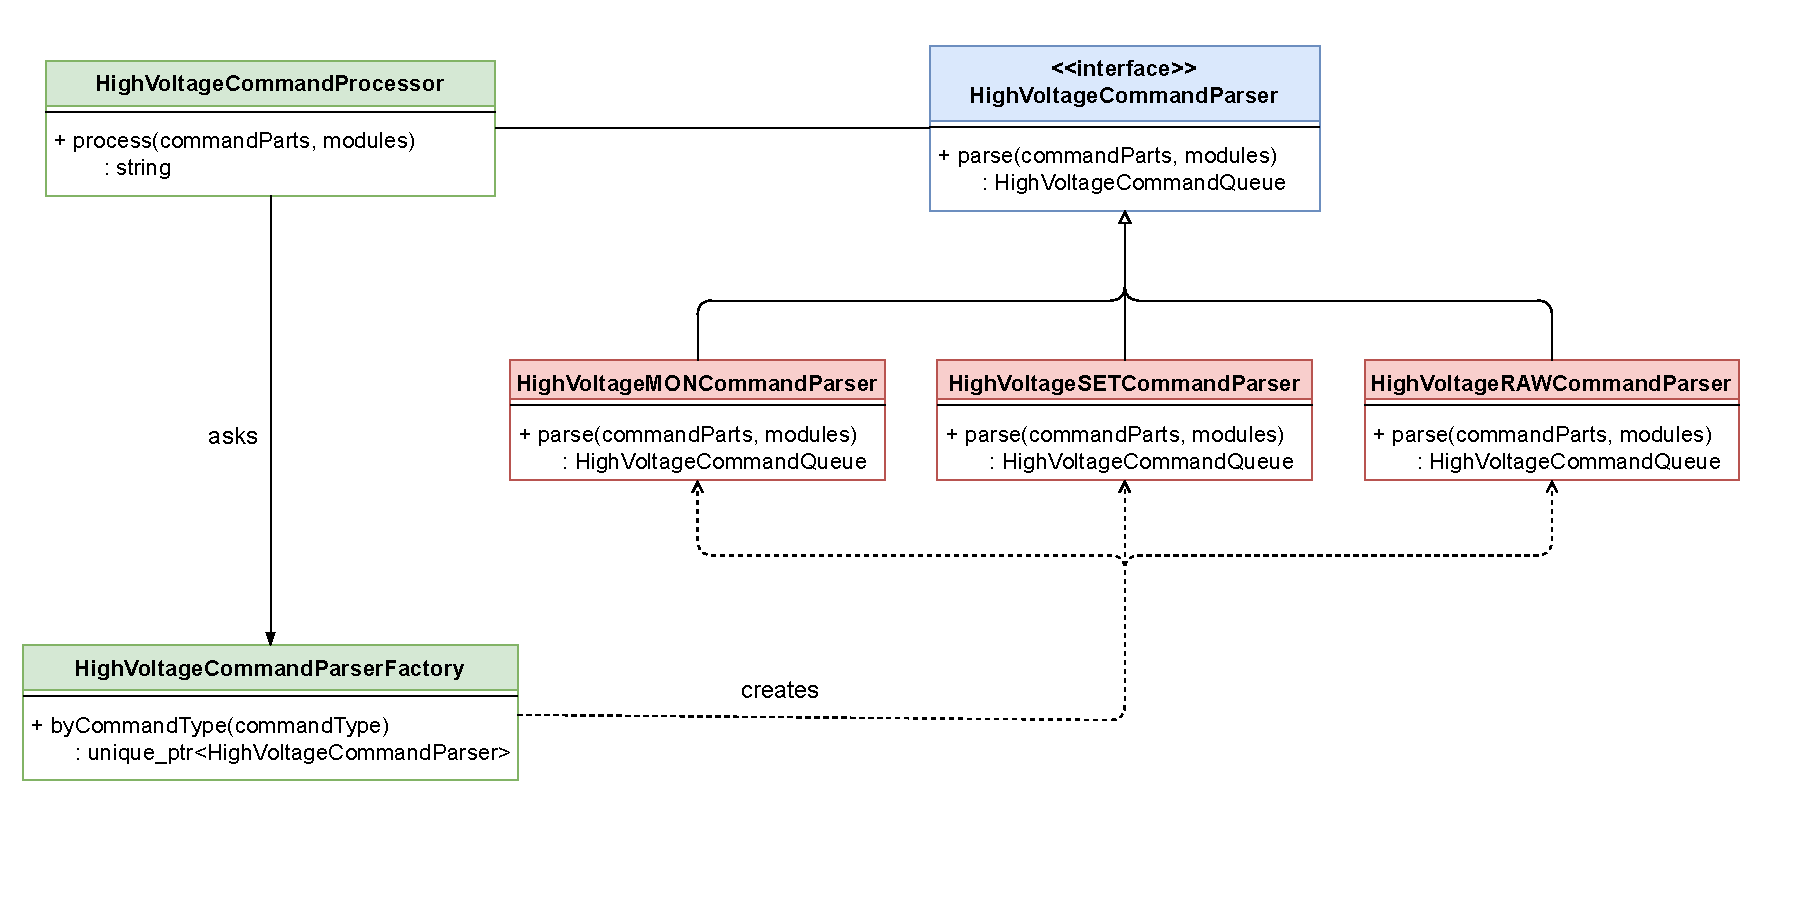
\includegraphics[width=\textwidth]{parsers.pdf}
\caption{Diagram klas obrazujący architekturę przygotowanej biblioteki: główną część stanowi oparta o polimorfizm hierarchia klas służących do przekształcania komend do zbioru obiektów reprezentujących czynności wykonywane na urządzeniach. }
\label{fig:psu_parsers}
\end{figure}

Obiekty reprezentujące poszczególne czynności wykonywane na urządzeniach, przechowywane w zapełnianym przez parsery kontenerze \lstinline{HighVoltageCommandQueue}, również modelowane są przez polimorficzną hierarchię klas (rys. \ref{fig:psu_commands}). Poszczególne klasy dziedziczące po abstrakcji \lstinline{HighVoltageCommand} odpowiadają za: czynności wykonywane na pojedynczym urządzeniu, pojedynczym kanale oraz komendy typu RAW.

\begin{figure}[H]
\centering
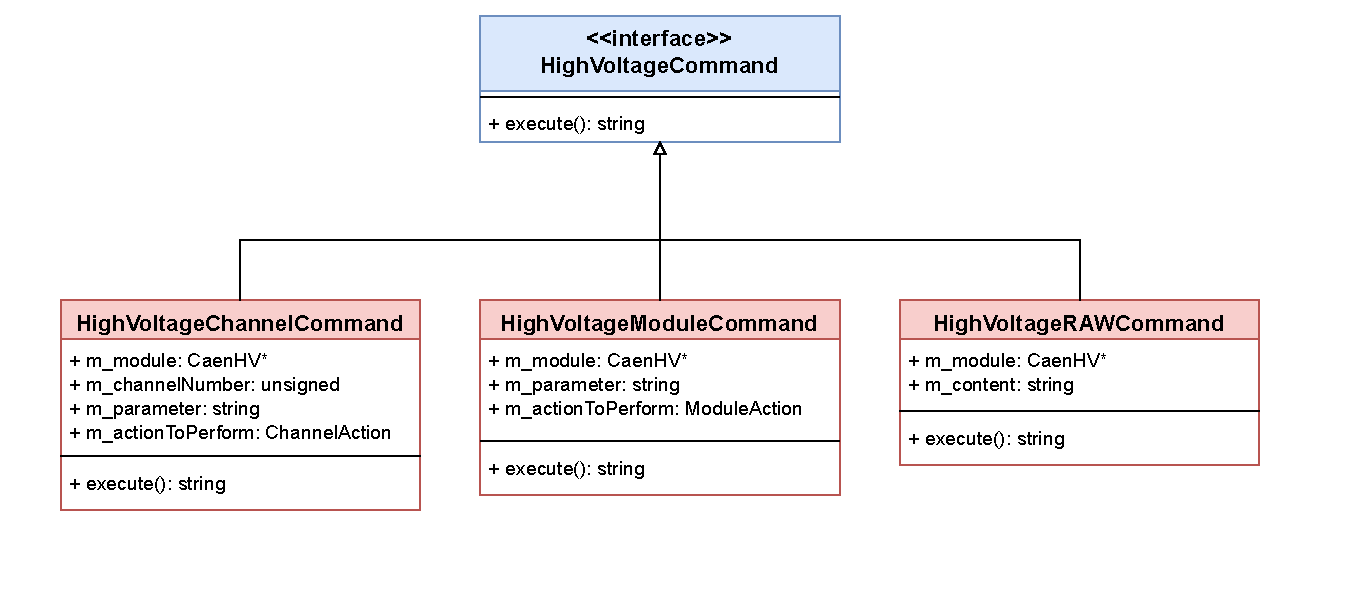
\includegraphics[width=\textwidth]{commands.pdf}
\caption{Diagram klas obrazujący hierarchię reprezentującą czynności wykonywane na urządzeniach.}
\label{fig:psu_commands}
\end{figure}

Dla biblioteki przygotowane zostały testy jednostkowe, pozwalające na automatyczną weryfikację poprawności implementacji. Ponadto przygotowane komendy były wielokrotnie testowane w środowisku produkcyjnym (co jest szczególnie istotne z uwagi na ich ścisły związek z urządzeniami), co zostało opisane w części pracy poświęconej testom projektu.

\clearpage
\subsection{Rozbudowa biblioteki odpowiedzialnej za dopasowywanie krzywej}

\clearpage
\subsection{Zmiany w sposobie aktualizacji parametrów i zebranych danych}
W swojej oryginalnej wersji system GGSS nie udostępniał możliwości aktualizacji niektórych parametrów oraz zebranych danych na żądanie - następowało to jedynie w ściśle określonych momentach działania systemu, takich jak zakończenie pomiaru za pomocą danego licznika słomkowego. Zadaniem autorów była rozbudowa projektu o możliwość aktualizacji na żądanie parametrów, takich jak monitorowane na danym liczniku napięcie, oraz danych w postaci zebranego widma.

Aktualizacja parametrów na żądanie osiągnięta została za pomocą komend wysyłanych przez użytkownika za pośrednictwem protokołu DIM. Istniejąca w oryginalnej wersji projektu komenda \lstinline{update} dokonywała jedynie przesłania do systemu WinCC OA znajdującej się w pamięci struktury. Autorzy rozbudowali ją o wywołanie funkcji \lstinline{UpdateAllCurrentlyMeasuredChannelsHVData}, która przed wysłaniem informacji dokonuje aktualizacji danych związanych z wykorzystywanymi w projekcie zasilaczami wysokiego napięcia poprzez wykonanie zapytania za pomocą dostarczonych przez producenta urządzenia komend. Pozyskiwane w ten sposób dane to: monitorowane oraz ustawione napięcie oraz monitorowane natężenie prądu - w przypadku dwóch pierwszych parametrów wynikowe wartości możliwe są do zaobserwowania na dostępnym w systemie WinCC OA panelu (rys. \ref{fig:hv_params}).

\begin{figure}[H]
\centering
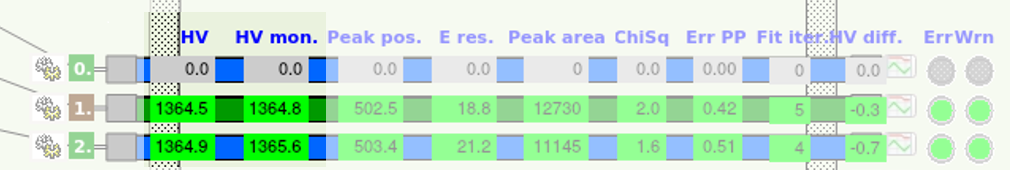
\includegraphics[width=\textwidth]{params_hv.png}
\caption{Fragment panelu dostępnego w ramach technologii WinCC OA, zawierającego dane dotyczące wykorzystywanych w systemie liczników słomkowych. Charakteryzujący się mniejszą przezroczystością fragment rysunku zawiera parametry \emph{HV} oraz \emph{HV mon.}, mogące podlegać aktualizacji dzięki wprowadzonym przez autorów zmianom.}
\label{fig:hv_params}
\end{figure}

Działanie najnowszej wersji komendy \lstinline{update} zaprezentowane zostało na rysunku \ref{fig:hv_on_demand} - przedstawia on fragmenty dwóch paneli dostępnych w ramach systemu WinCC OA. Panel znajdujący się po prawej stronie rysunku służy to wysyłania do systemu GGSS komend za pomocą protokołu DIM. Przedstawiony zrzut ekranu wykonany został w krótkim czasie po uruchomieniu aplikacji, przed zakończeniem pierwszego wykonywanego pomiaru - stąd widoczne są wartości 0.0. Po wykonaniu komendy \lstinline{update} dokonana została natomiast aktualizacja, w wyniku której pozyskane zostały aktualne wartości napięć dla wszystkich wykorzystanych kanałów - dzięki temu możliwa była obserwacja wartości dla kanału oznaczonego numerem 3, za pomocą którego wykonywany był w danym momencie pomiar, a zatem napięcie zostało znacznie zwiększone. W pierwotnej wersji systemu wykonanie polecenia \lstinline{update} nie spowodowałoby aktualizacji tych wartości - miałoby to miejsce dopiero po zakończeniu pomiaru na kanale numer 3.

\begin{figure}[H]
\centering
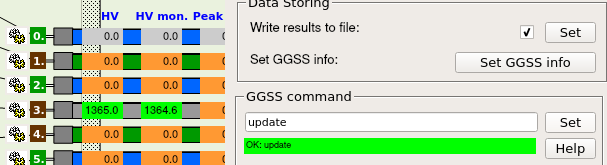
\includegraphics[width=\textwidth]{on_demand.png}
\caption{Fragmenty dwóch paneli dostępnych w ramach technologii WinCC OA. Widoczna jest wysoka wartość napięcia odnotowana dla kanału numer 3 po wykonaniu komendy \lstinline{update}. W swojej oryginalnej wersji zaprezentowane polecenie nie dokonałoby aktualizacji parametrów związanych z zasilaczami wysokiego napięcia.}
\label{fig:hv_on_demand}
\end{figure}

W systemie istnieje ponadto polecenie \lstinline{update channel <kanał>}, pozwalające dokonać aktualizacji tylko dla jednego, wybranego licznika. Zostało ono w podobny sposób rozbudowane przez autorów o funkcjonalność aktualizacji wartości parametrów związanych z pracą zasilaczy wysokiego napięcia. Fragment przygotowanego przez autorów kodu, odpowiedzialnego za pozyskanie od zasilacza odpowiednich danych i umieszczenie ich w strukturze przesyłanej za pomocą protokołu DIM, przedstawiony został na listingu \ref{lst:on_demand}.

\lstinputlisting[
    language=C++, 
    caption={Fragment kodu wchodzącego w skład biblioteki \emph{ggss-lib}, którego zadaniem jest pobranie aktualnych wartości napięć i natężenia prądu dla pojedynczego kanału zasilacza oraz umieszczenie ich w strukturze używanej do komunikacji za pomocą protokołu DIM.}, 
    label={lst:on_demand}
]{5_code/code_samples/on_demand.cpp}

W najnowszej wersji systemu aktualizacja parametrów dla wszystkich kanałów biorących udział w pomiarach wykonywana jest ponadto po uruchomieniu systemu (ang. \emph{on start}) - w oryginalnej wersji systemu po uruchomieniu aplikacji, aby otrzymać dane, należało odczekać do zakończenia pierwszego pomiaru wykonywanego za pomocą danego licznika słomkowego. System wykonuje aktualizację również za każdym razem, gdy otrzyma od użytkownika poprawną komendę SET modyfikującą parametry zasilaczy wysokiego napięcia.

Autorzy rozszerzyli aplikację \lstinline{ggss-runner} o szereg komend pozwalających użytkownikowi na prowadzenie zaawansowanej interakcji z systemem. Najważniejsze z nich to:
\begin{itemize}
\item \lstinline{update all_straws} - dokonuje aktualizacji parametrów dla wszystkich liczników słomkowych, niezależnie od tego czy są one używane do wykonywania pomiarów
\item \lstinline{update spectrum} - dokonuje aktualizacji na żądanie widma zebranego przy pomocy licznika słomkowego wykorzystywanego w danym momencie do wykonywania pomiaru, 
\item \lstinline{update all} - kombinacja komend \lstinline{update} i \lstinline{update spectrum}
\end{itemize}

Z punktu widzenia niniejszej pracy szczególnie istotne jest polecenie \lstinline{update spectrum}, pozwalające pozyskać zebrane do momentu jego wykonania dane (widmo) dla kanału aktualnie używanego do przeprowadzania pomiaru. W pierwotnej wersji systemu GGSS nie istniała możliwość uzyskania zebranych danych przed zakończeniem pomiaru wykonywanego za pomocą danego licznika słomkowego. Ponieważ czas trwania pojedynczego pomiaru może sięgać nawet 10 minut, konieczne było zaimplementowanie mechanizmu pozwalającego użytkownikowi zobaczyć zebrane dane w czasie jego trwania. Przykład zastosowania przygotowanego polecenia przedstawiony został na rysunku \ref{fig:spectrum_update}.

\begin{figure}[H]
\centering

\begin{subfigure}{0.66\textwidth}
\centering
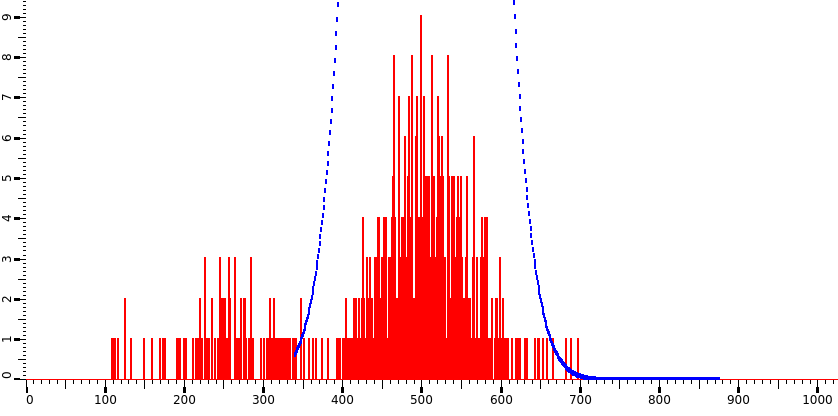
\includegraphics[width=\textwidth]{spectrum_update_1.png}
\caption{Efekt pierwszego wywołania komendy \lstinline{update spectrum} - widoczna niewielka ilość zebranych przez system danych.}
\label{fig:spectrum_update_1}
\end{subfigure}

\vspace*{8pt}%

\begin{subfigure}{0.66\textwidth}
\centering
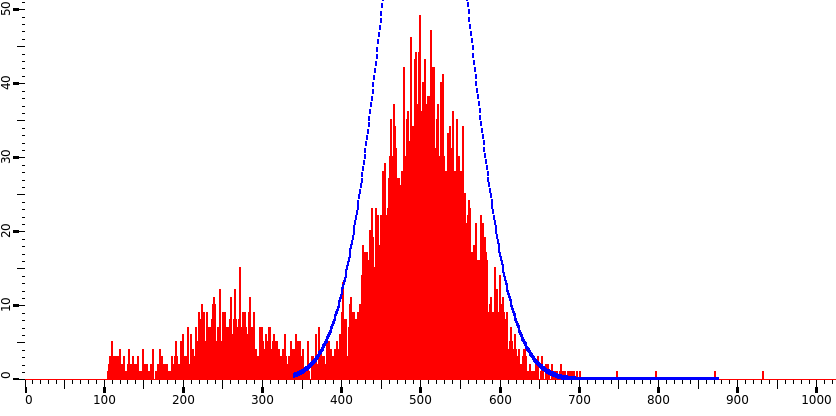
\includegraphics[width=\textwidth]{spectrum_update_2.png}
\caption{Efekt drugiego wywołania komendy \lstinline{update spectrum} - widoczna większa ilość danych niż w przypadku wywołania pierwszego.}
\label{fig:spectrum_update_2}
\end{subfigure}

\caption{Przykład aktualizacji na żądanie zebranych danych: fragment panelu przedstawiającego dane w postaci histogramu, dla dwóch następujących po sobie w pewnym odstępie czasu użyć komendy \lstinline{update spectrum}.}
\label{fig:spectrum_update}
\end{figure}

\clearpage
\subsection{Zabezpieczenie przed przepełnieniem bufora urządzenia MCA}
Zbierane przez system GGSS dane, przed przekształceniem ich do postaci histogramu, przechowywane są w buforze urządzenia MCA dokonującego pomiar. Stosowana w projekcie konfiguracja pozwala na jednoczesne przechowywanie informacji o około 30000 zliczeniach. Przeprowadzane testy wykazały, że dla pewnych konfiguracji projektu liczba ta nie jest wystarczająca - zaprezentowane zostało to na rysunku \ref{fig:mca_1}, gdzie wartość \emph{Peak area}, stanowiąca sumę liczebności przedziałów histogramu w pobliżu maksimum lokalnego, wynosi 27235 dla licznika o numerze 3. Niezależnie od zwiększania czasu trwania pomiaru, wartość ta nie ulegała zwiększeniu, ponieważ nowe dane były odrzucane z powodu przepełnienia wspomnianego już bufora. Należy zaznaczyć, że rozwiązanie zaprezentowanego problemu musiało zostać zrealizowane po stronie warstwy oprogramowania systemu - jakiekolwiek zmiany w warstwie sprzętowej nie były na tym etapie możliwe.

\begin{figure}[H]
\centering
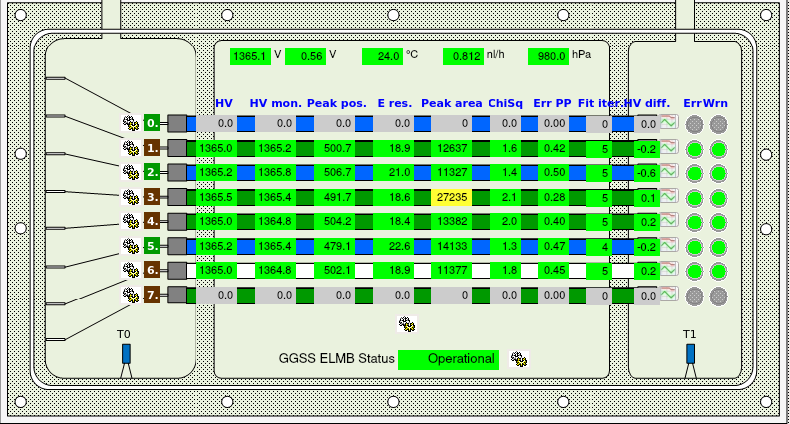
\includegraphics[width=\textwidth]{mca_1.png}
\caption{Przykład prezentujący problem przepełnienia bufora urządzenia MCA: dla odpowiednio długiego czasu trwania pomiaru wartość \emph{Peak area} dla licznika słomkowego oznaczonego numerem 3 osiąga wartość 27000 i nie ulega zwiększeniu wraz z wydłużaniem czasu zbierania danych.}
\label{fig:mca_1}
\end{figure}

Przygotowane przez autorów rozwiązanie oparte zostało na okresowym przenoszeniu danych zawartych w buforze urządzenia MCA do znajdującej się w pamięci RAM komputera struktury. Dzięki temu wspomniany bufor może być regularnie opróżniany, co chroni przed jego przepełnieniem. W pierwotnej wersji systemu, po rozpoczęciu pomiaru odpowiedzialny za niego wątek przechodził w stan oczekiwania na zakończenie operacji (lub otrzymanie sygnału STOP zatrzymującego zbieranie danych). Zaproponowana przez autorów modyfikacja polega na podziale czasu oczekiwania na mniejsze odcinki, na końcu których zebrane dane przenoszone są do pamięci RAM. Uproszczona na potrzeby niniejszego manuskryptu implementacja tego algorytmu zaprezentowana została na listingu \ref{lst:mca} - stosowany w projekcie algorytm uwzględnia ponadto kilka dodatkowych aspektów działania systemu, takich jak konieczność dokonania w połowie trwania pomiaru aktualizacji urządzenia ELMB za pośrednictwem systemu WinCC OA i protokołu DIM.

\lstinputlisting[
    language=C++, 
    caption={Uproszczona na potrzeby manuskryptu implementacja rozwiązania problemu przepełniającego się bufora - w określonych odstępach czasu wywoływana jest funkcja \lstinline{GetData}, której działanie polega na przeniesieniu danych znajdujących się w buforze urządzenia MCA do pamięci RAM, przy jednoczesnym jego opróżnieniu.}, 
    label={lst:mca}
]{5_code/code_samples/mca.cpp}

Okres wykonywania operacji przenoszenia zebranych danych określany jest w sekundach za pomocą parametru \lstinline{mcaRefreshInterval}, który może zostać umieszczony w pliku konfiguracyjnym lub przekazany do systemu za pomocą komendy. W celu zachowania kompatybilności wstecznej z poprzednimi wersjami projektu parametr ten jest opcjonalny - jego brak lub przypisanie mu wartości 0 oznacza działanie systemu bez wprowadzonej poprawki (fladze \lstinline{shouldRefreshMca} przypisywana jest w takim wypadku wartość \lstinline{false}). Aby pobrać wartość tego parametru należy za pomocą protokołu DIM wysłać do systemu komendę \lstinline{get mcaRefreshInterval}. Modyfikacja jego wartości wykonywana jest natomiast za pomocą polecenia \lstinline{set ggss parameter mcaRefreshInterval value <oczekiwana_wartość>}. 

Przygotowane rozwiązanie zostało przez autorów poddane testom w środowisku docelowym. Na rysunku \ref{fig:mca_2} przedstawione zostało działanie systemu GGSS w sytuacji, gdy parametr \lstinline{mcaRefreshInterval} przyjmuje wartość niezerową - bufor urządzenia MCA nie ulega przepełnieniu, o czym świadczy wysoka (przekraczająca 32768) wartość parametru \emph{Peak area} dla danych zebranych za pomocą liczników słomkowych oznaczonych numerami 2 oraz 4.

\begin{figure}[H]
\centering
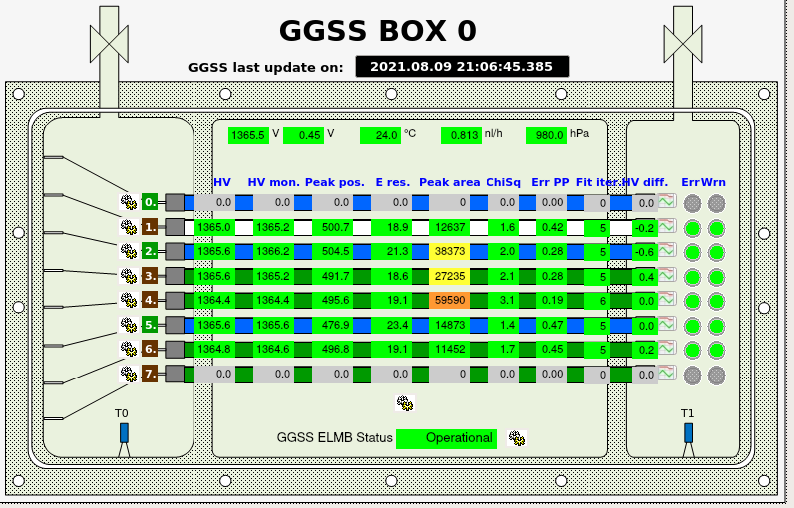
\includegraphics[width=\textwidth]{mca_2.png}
\caption{Działanie systemu GGSS po wprowadzeniu przez autorów rozszerzenia jego możliwości o cykliczne przenoszenie zebranych danych z bufora urządzenia MCA do pamięci RAM komputera. W przypadku liczników oznaczonych numerami 2 oraz 4 widoczna jest przekraczająca wartość 32768 liczba zliczeń, co świadczy o tym, że nie dochodzi do przepełnienia wspomnianego bufora.}
\label{fig:mca_2}
\end{figure}

\subsection{Możliwość przywracania domyślnej kolejności liczników słomkowych}

Kolejność, w jakiej poszczególne liczniki słomkowe wykorzystywane są do przeprowadzania pomiarów, stanowi możliwy do modyfikacji przez użytkownika parametr systemu GGSS. Manipulowanie nim możliwe było już w oryginalnej wersji projektu. Autorzy wprowadzili jednak dodatkowo możliwość zapamiętania jego oryginalnej, odczytanej z pliku konfiguracyjnego, wartości, dzięki czemu możliwe jest jej przywrócenie. Służy do tego dodana do systemu komenda \lstinline{reset channelsOrder}, którą wykonać można, gdy aplikacja nie przeprowadza żadnych pomiarów (tzn. gdy system znajduje się w stanie zatrzymania). Na potrzeby zilustrowania tej funkcjonalności rozważony zostanie przykład, w którym aplikacja uruchamiana jest z domyślną kolejnością ustaloną jako \lstinline{0:3,0:6,0:4,0:2,0:5,0:1}. Następnie użytkownik za pomocą specjalnego panelu (rys. \ref{fig:order_change}) dokonuje zmiany kolejności na obejmującą mniejszą liczbę liczników słomkowych: \lstinline{0:3,0:6,0:4}.


\begin{figure}[H]
\centering
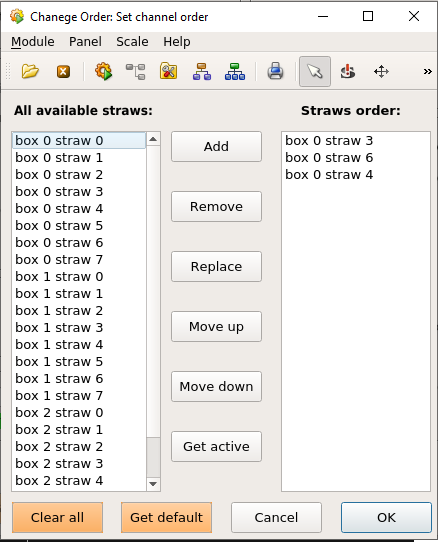
\includegraphics[width=0.4\textwidth]{order_change.png}
\caption{Dostępny w ramach infrastruktury WinCC OA panel pozwalający na modyfikację kolejności, w jakiej poszczególne liczniki słomkowe wykorzystywane są do przeprowadzania pomiarów.}
\label{fig:order_change}
\end{figure}


Po zmianie kolejności użytkownik dokonuje próby przywrócenia jej domyślnej wartości za pomocą komendy \lstinline{reset channelsOrder} - w zależności od tego, czy system GGSS jest w tym momencie zatrzymany, komenda ta zwróci błąd (gdy nie jest - rys. \ref{fig:order_com_1}) lub wynik pozytywny (gdy jest - rys. \ref{fig:order_com_2}). Ponadto użytkownik ma możliwość sprawdzenia w dowolnym momencie przechowywanej w systemie wartości - służy do tego komenda \lstinline{get defaultChannelsOrder}, której działanie zaprezentowane zostało na rysunku \ref{fig:order_com_3}. Funkcjonalność ta została ponadto zintegrowana w postaci przycisku \emph{Get default} z przedstawionym na rys. \ref{fig:order_change} panelem. Autorzy nie brali jednak bezpośredniego udziału w rozwoju infrastruktury opartej o technologię WinCC OA - podczas przeprowadzania wspomnianej integracji pełnili jedynie rolę konsultacyjną.

\begin{figure}[H]
\centering

\begin{subfigure}{0.45\textwidth}
\centering
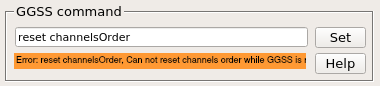
\includegraphics[width=\textwidth]{reset_order_1.png}
\caption{Błąd wykonania komendy resetującej.}
\label{fig:order_com_1}
\end{subfigure}
\begin{subfigure}{0.45\textwidth}
\centering
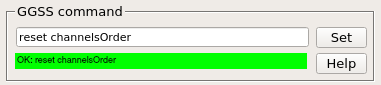
\includegraphics[width=\textwidth]{reset_order_2.png}
\caption{Poprawne wykonanie komendy resetującej.}
\label{fig:order_com_2}
\end{subfigure}

\vspace*{8pt}%

\begin{subfigure}{0.45\textwidth}
\centering
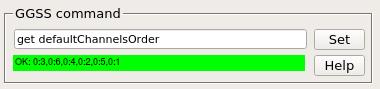
\includegraphics[width=\textwidth]{get_order.png}
\caption{Działanie komendy pozwalającej na pobranie domyślnej kolejności.}
\label{fig:order_com_3}
\end{subfigure}

\caption{Przykłady zastosowania przesyłanych do systemu GGSS za pomocą protokołu DIM komend służących do operacji na domyślnej kolejności, w jakiej poszczególne liczniki słomkowe wykorzystywane są do przeprowadzania pomiarów.}
\label{fig:order_com}
\end{figure}


\subsection{Pomniejsze rozszerzenia}
Poza opisanymi do tej pory zmianami, autorzy wprowadzili w projekcie kilka pomniejszych rozszerzeń - przykładem tego typu modyfikacji jest rozbudowa możliwości biblioteki \emph{caenhv-lib}, odpowiedzialnej za wysokopoziomową implementację komunikacji z zasilaczami wysokiego napięcia. Zmiana ta polegała przede wszystkim na umożliwieniu pozyskiwania i modyfikowania większej liczby parametrów urządzeń. W pierwotnej wersji biblioteka pozwalała jedynie na uzyskanie najbardziej istotnych informacji, takich jak wartość monitorowanego na danym kanale napięcia. Wykorzystywane w projekcie zasilacze CAEN N1470 oferują natomiast bardzo rozbudowaną możliwość konfiguracji, obejmującą m.in. prędkość przyrostu i spadku napięcia po dokonaniu zmiany jego oczekiwanej wartości. Autorzy rozbudowali więc bibliotekę o dodatkowe funkcje pozwalające na manipulację tego typu parametrami. Zmiana ta jest istotna z punktu widzenia opisanej w sekcji \ref{ch:hv} biblioteki obsługującej komendy wysyłane do zasilaczy - w celu wykonania operacji na urządzeniu wykorzystuje ona bowiem obiekty klas udostępnianych przez bibliotekę \emph{caenhv-lib}. W swojej aktualnej wersji poddana rozbudowie biblioteka wspiera niemal wszystkie udostępniane przez producenta parametry zasilaczy.
